\documentclass[12pt]{article}

\usepackage[T1]{fontenc}
\usepackage[utf8]{inputenc}
\usepackage[italian]{babel}
\usepackage{fancyhdr}
\usepackage[margin=2cm]{geometry}
\usepackage{tocloft}
\usepackage{amsmath}
\usepackage{enumitem}
\usepackage{graphicx}

\renewcommand{\cftsecleader}{\cftdotfill{\cftdotsep}}
\renewcommand{\thesection}{\arabic{section}.}
\renewcommand{\thesubsection}{\arabic{section}.\arabic{subsection}}

\setlength{\headheight}{15pt}

\pagestyle{fancy}
\renewcommand{\footrulewidth}{0.4pt}
\lhead{\bfseries Requisiti di sistema}
\chead{}
\rhead{}
\lfoot{}
\cfoot{}
\rfoot{\thepage}


\begin{document}
\begin{titlepage}
   \begin{center}
       \vspace*{4cm}
 
       \textbf{\Huge{Riconoscitore di grammatiche LR(1)}}
 
       \vspace{0.5cm}
        \large{Manuale di utilizzo}
 
       \vspace{2cm}
 
       \textbf{Luca Filice, Matteo Gusmini, Davide Presciani}
 
       \vfill
 
       
\includegraphics[width=0.4\textwidth]{immagini/logo}
 
       Università degli Studi di Bergamo\\
       Dipartimento di Ingegneria Gestionale, dell'Informazione e della trasmissione\\
 
   \end{center}
\end{titlepage}
\tableofcontents

\pagebreak

\section{Introduzione}
Il seguente documento illustra il manuale di utilizzo del riconoscitore di grammatiche LR(1).

\section{Struttura corretta della grammatica}\label{struttura}
Il programma deve riconoscere come formalmente corrette (quindi prive di errori sintattici, lessicali e/o grammaticali) soltanto grammatiche che presentino la seguente struttura:
\begin{itemize}
\item una prima regola $pr$ che abbia come elemento di sinistra il non terminale $S0$, definita come segue
$$
SZ \hspace{5pt} EQ \hspace{5pt} NT \hspace{5pt} TER \hspace{5pt} SC
$$
\item altre $n \geq 1$ regole di produzione $ar$, che formano il resto della grammatica, definite come segue
$$
NT \hspace{5pt} EQ \hspace{5pt} \left( NT \left| CT \right. \right)^* \hspace{5pt} SC
$$
\end{itemize}
I blocchi componenti le regole appena definite sono così traducibili:
\begin{table}[h]
\centering
\begin{tabular}{|c|c|}
\hline
\textbf{Simbolo} & \textbf{Caratteri} \\
\hline
$SZ$ & $S0$ \\
\hline
$EQ$ & $-> \left| \hspace{5pt} := \right.$ \\
\hline
$NT$ & $A \hspace{5pt} \dots \hspace{5pt} Z$ \\
\hline
$CT$ & $a \hspace{3pt} \dots z \left| \hspace{3pt} 0 \hspace{3pt} \dots \hspace{3pt} 9 \hspace{3pt} \right| \hspace{3pt} + \hspace{3pt} \left| \hspace{3pt} - \hspace{3pt} \right| \hspace{3pt} * \hspace{3pt} \left| \hspace{3pt} / \right.$ \\
\hline
$TER$ & $\text{/swa} \hspace{5pt} \left| \hspace{5pt} \text{/cjswa} \right.$ \\
\hline
$SC$ & $;$ \\
\hline
\end{tabular}
\caption{Corrispondenza tra caratteri della grammatica e blocchi di definizione delle regole}
\end{table}

\underline{Nota:} Per la definizione della struttura delle regole è stata utilizzata la notazione formale di Backus-Naur estesa (EBNF).

\subsection{Errori lessicali}
L'utilizzo di qualsiasi carattere non riconducibile alla colonna "Caratteri" della Tabella 1 corrisponde a un errore lessicale.

\subsection{Errori sintattici}
Gli errori sintattici sono dati dal mancato rispetto della struttura delle regole $pr$ e $ar$ come definite nel paragrafo "Struttura corretta della grammatica" a pagina \pageref{struttura}.

\subsection{Errori semantici}
Gli errori semantici si verificano nei seguenti casi:
\begin{itemize}
\item nella grammatica è presente un carattere non terminale che non presenta regole di produzioni associate;
\item nella grammatica è presente una regola duplicata (\underline{nota bene} questo \underline{non} è un errore bloccante).
\end{itemize}

\subsection{Esempio di struttura corretta della grammatica}
Un esempio di struttura corretta della grammatica, che dovrà essere inserita all'interno di un file .txt per permetterne la sua analisi, è la seguente:
\begin{figure}[h!]
\centering
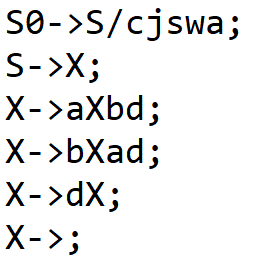
\includegraphics[scale=1.0]{immagini/esempioGrammatica.png}
\caption{Esempio di struttura corretta della grammatica}
\end{figure}

\underline{Easter Egg:} Il carattere terminatore può essere scritto come /swa (abbreviazione di swarrow, ossia il nome in LaTeX della classica freccia utilizzata come terminatore) oppure, come in questo caso, come /cjswa in onore del Capitan Jack Sparrow (per la somiglianza tra swarrow e Sparrow).


\section{Requisiti di sistema}
Il programma è eseguibile su più SO tra cui Windows, Linux e Mac OS. L'unico requisito necessario per l'utilizzo del programma è l'installazione del Java Development Kit oppure del Java Runtime Environment più recente.

\pagebreak

\section{Manuale di utilizzo}
\subsection{Selezione grammatica da analizzare}
All'avvio del programma ci si ritroverà davanti alla seguente pagina iniziale:
\begin{figure}[h!]
\centering
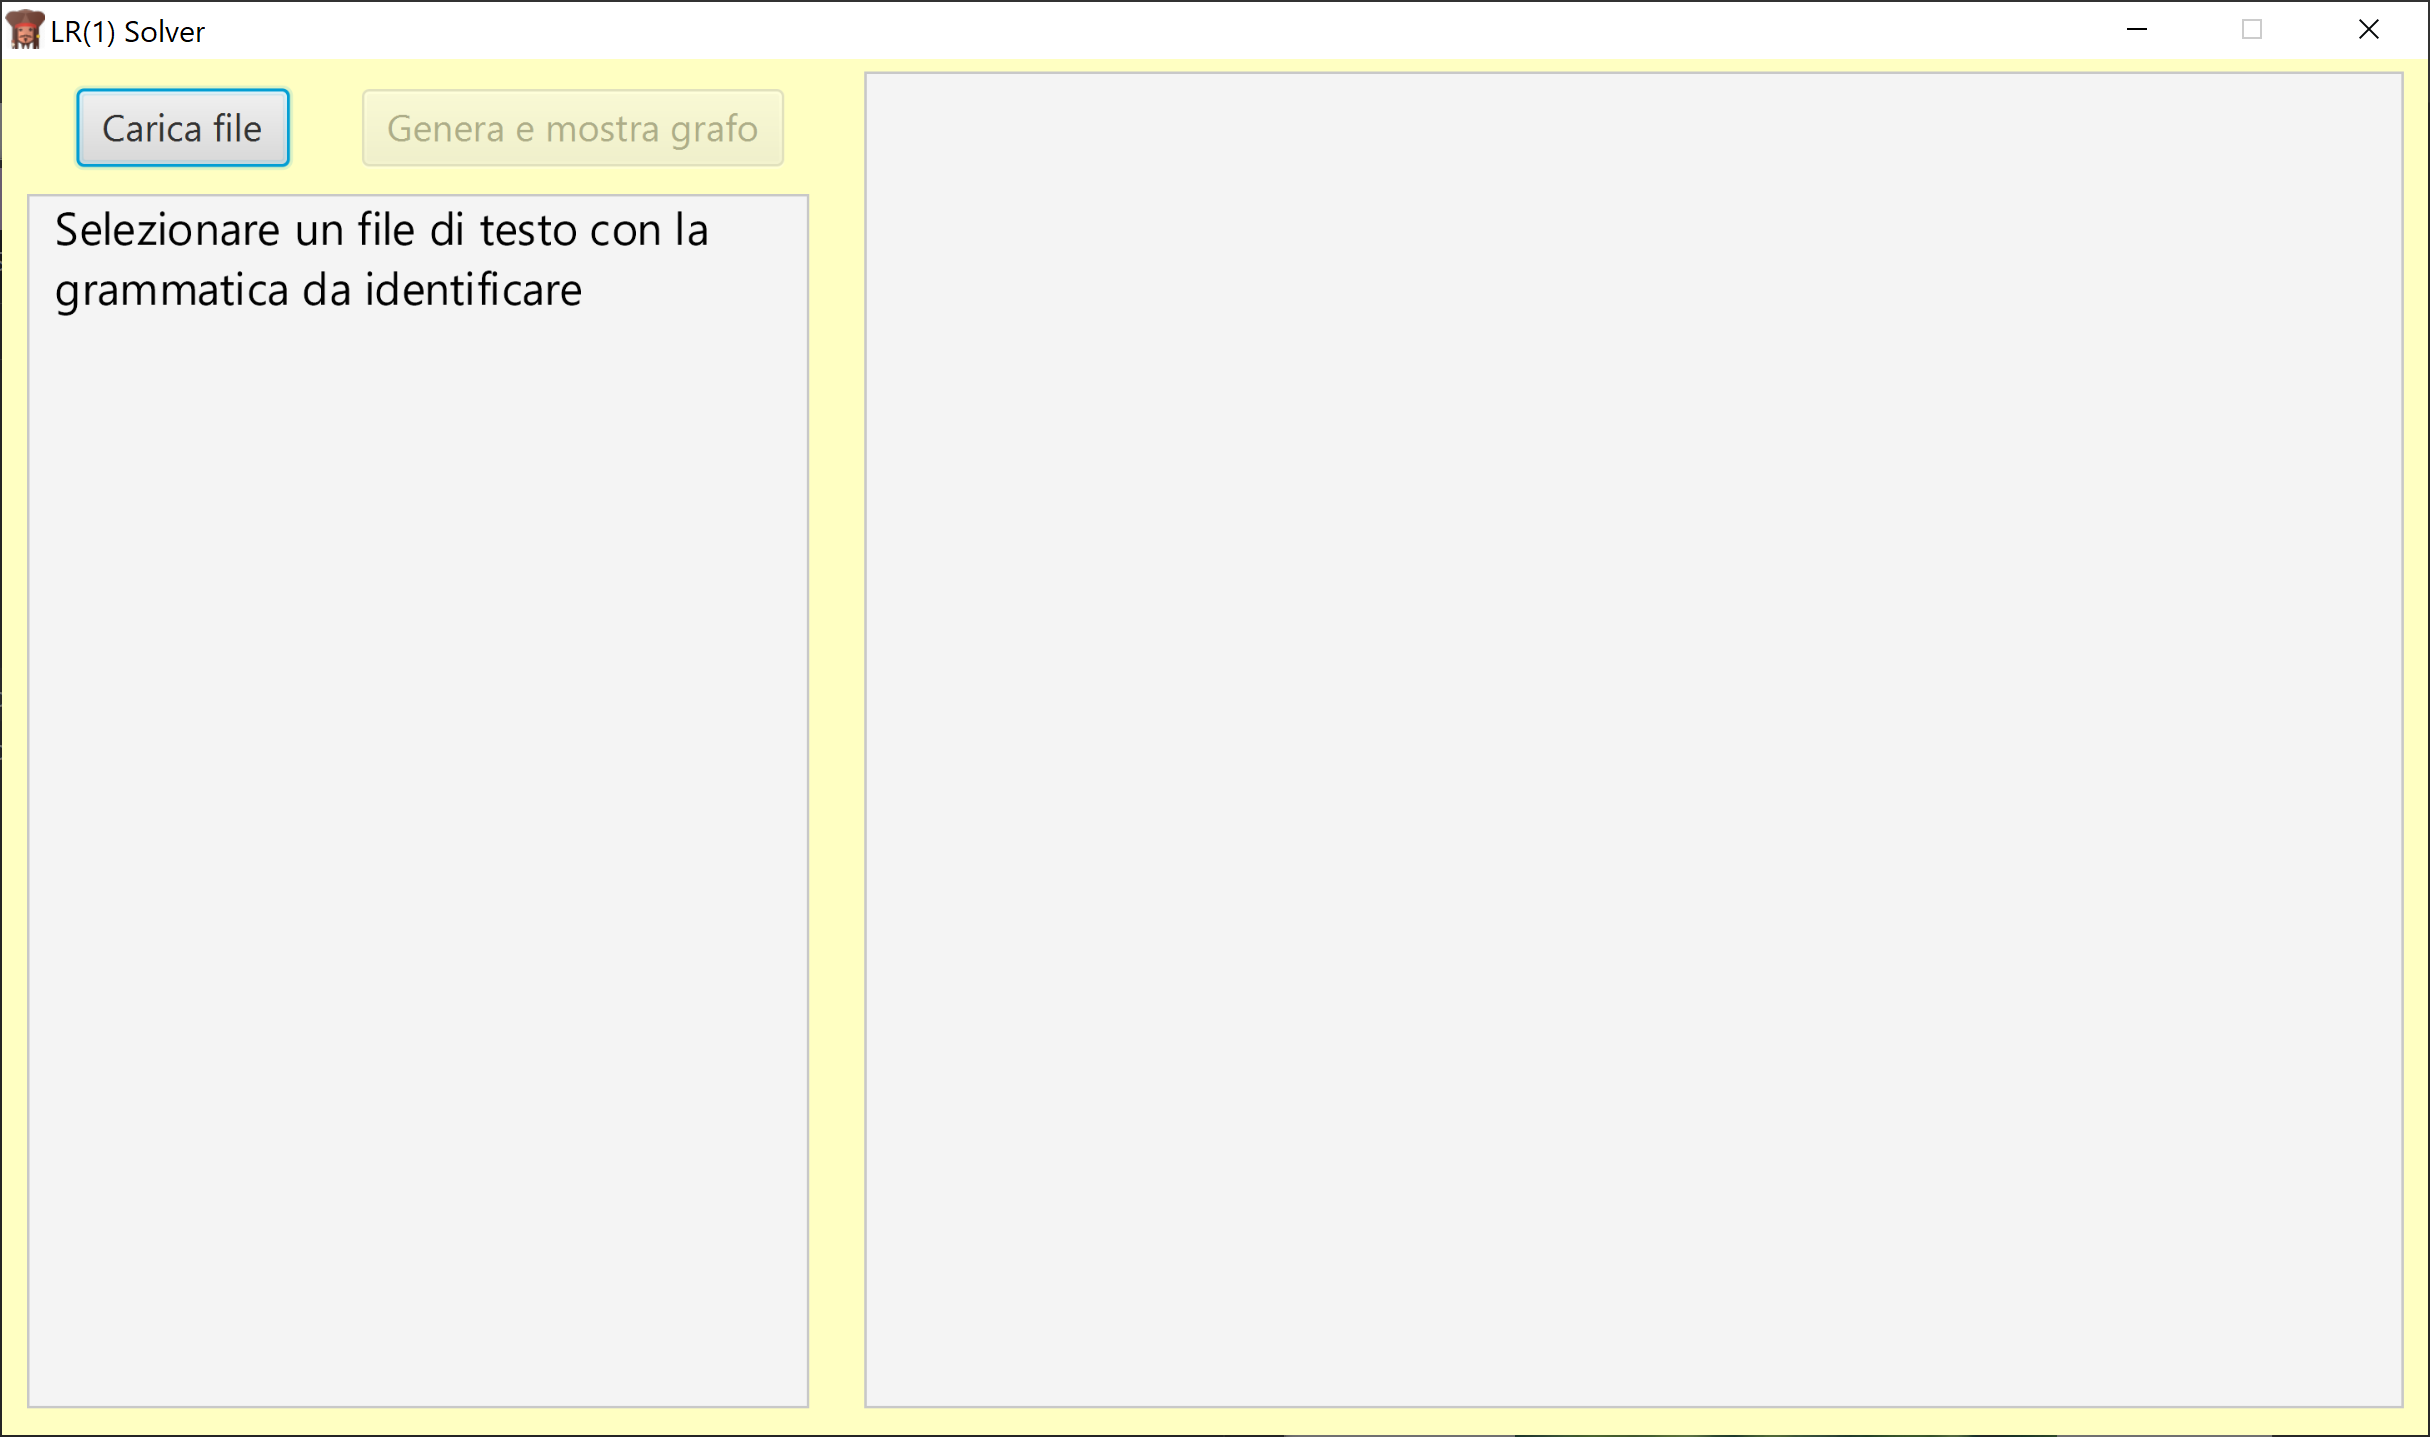
\includegraphics[scale=0.5]{immagini/Main.png}
\caption{Pagina iniziale}
\end{figure}

Da questa finestra è possibile premere il tasto "Carica file" per selezionare il file .txt con la grammatica da analizzare.
\begin{figure}[h!]
\centering
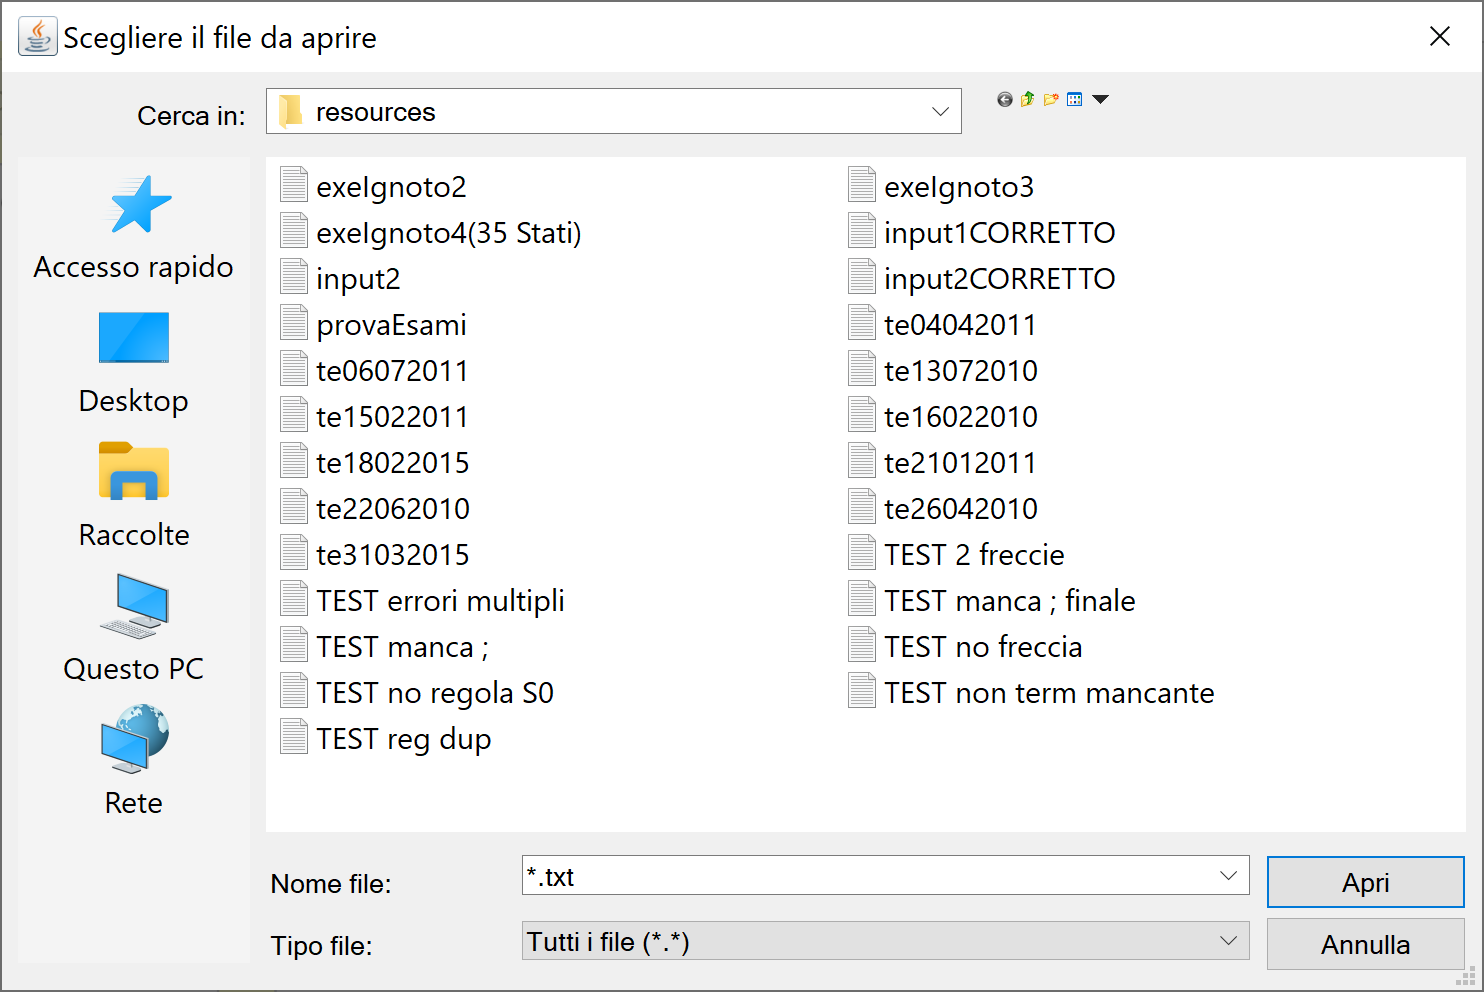
\includegraphics[scale=0.6]{immagini/SelezioneLinguaggio.png}
\caption{Finestra per la selezione del file}
\end{figure}

Una volta selezionato il file desiderato, il programma procederà all'analisi della grammatica, informando l'utente se essa sia o non sia di tipo LR(1) oppure se il file contenga degli errori.
\pagebreak

\subsection{Esempio grammatica LR(1)}
Se la grammatica inserita è di tipo LR(1) verrà visualizzato un messaggio come il seguente:
\begin{figure}[h!]
\centering
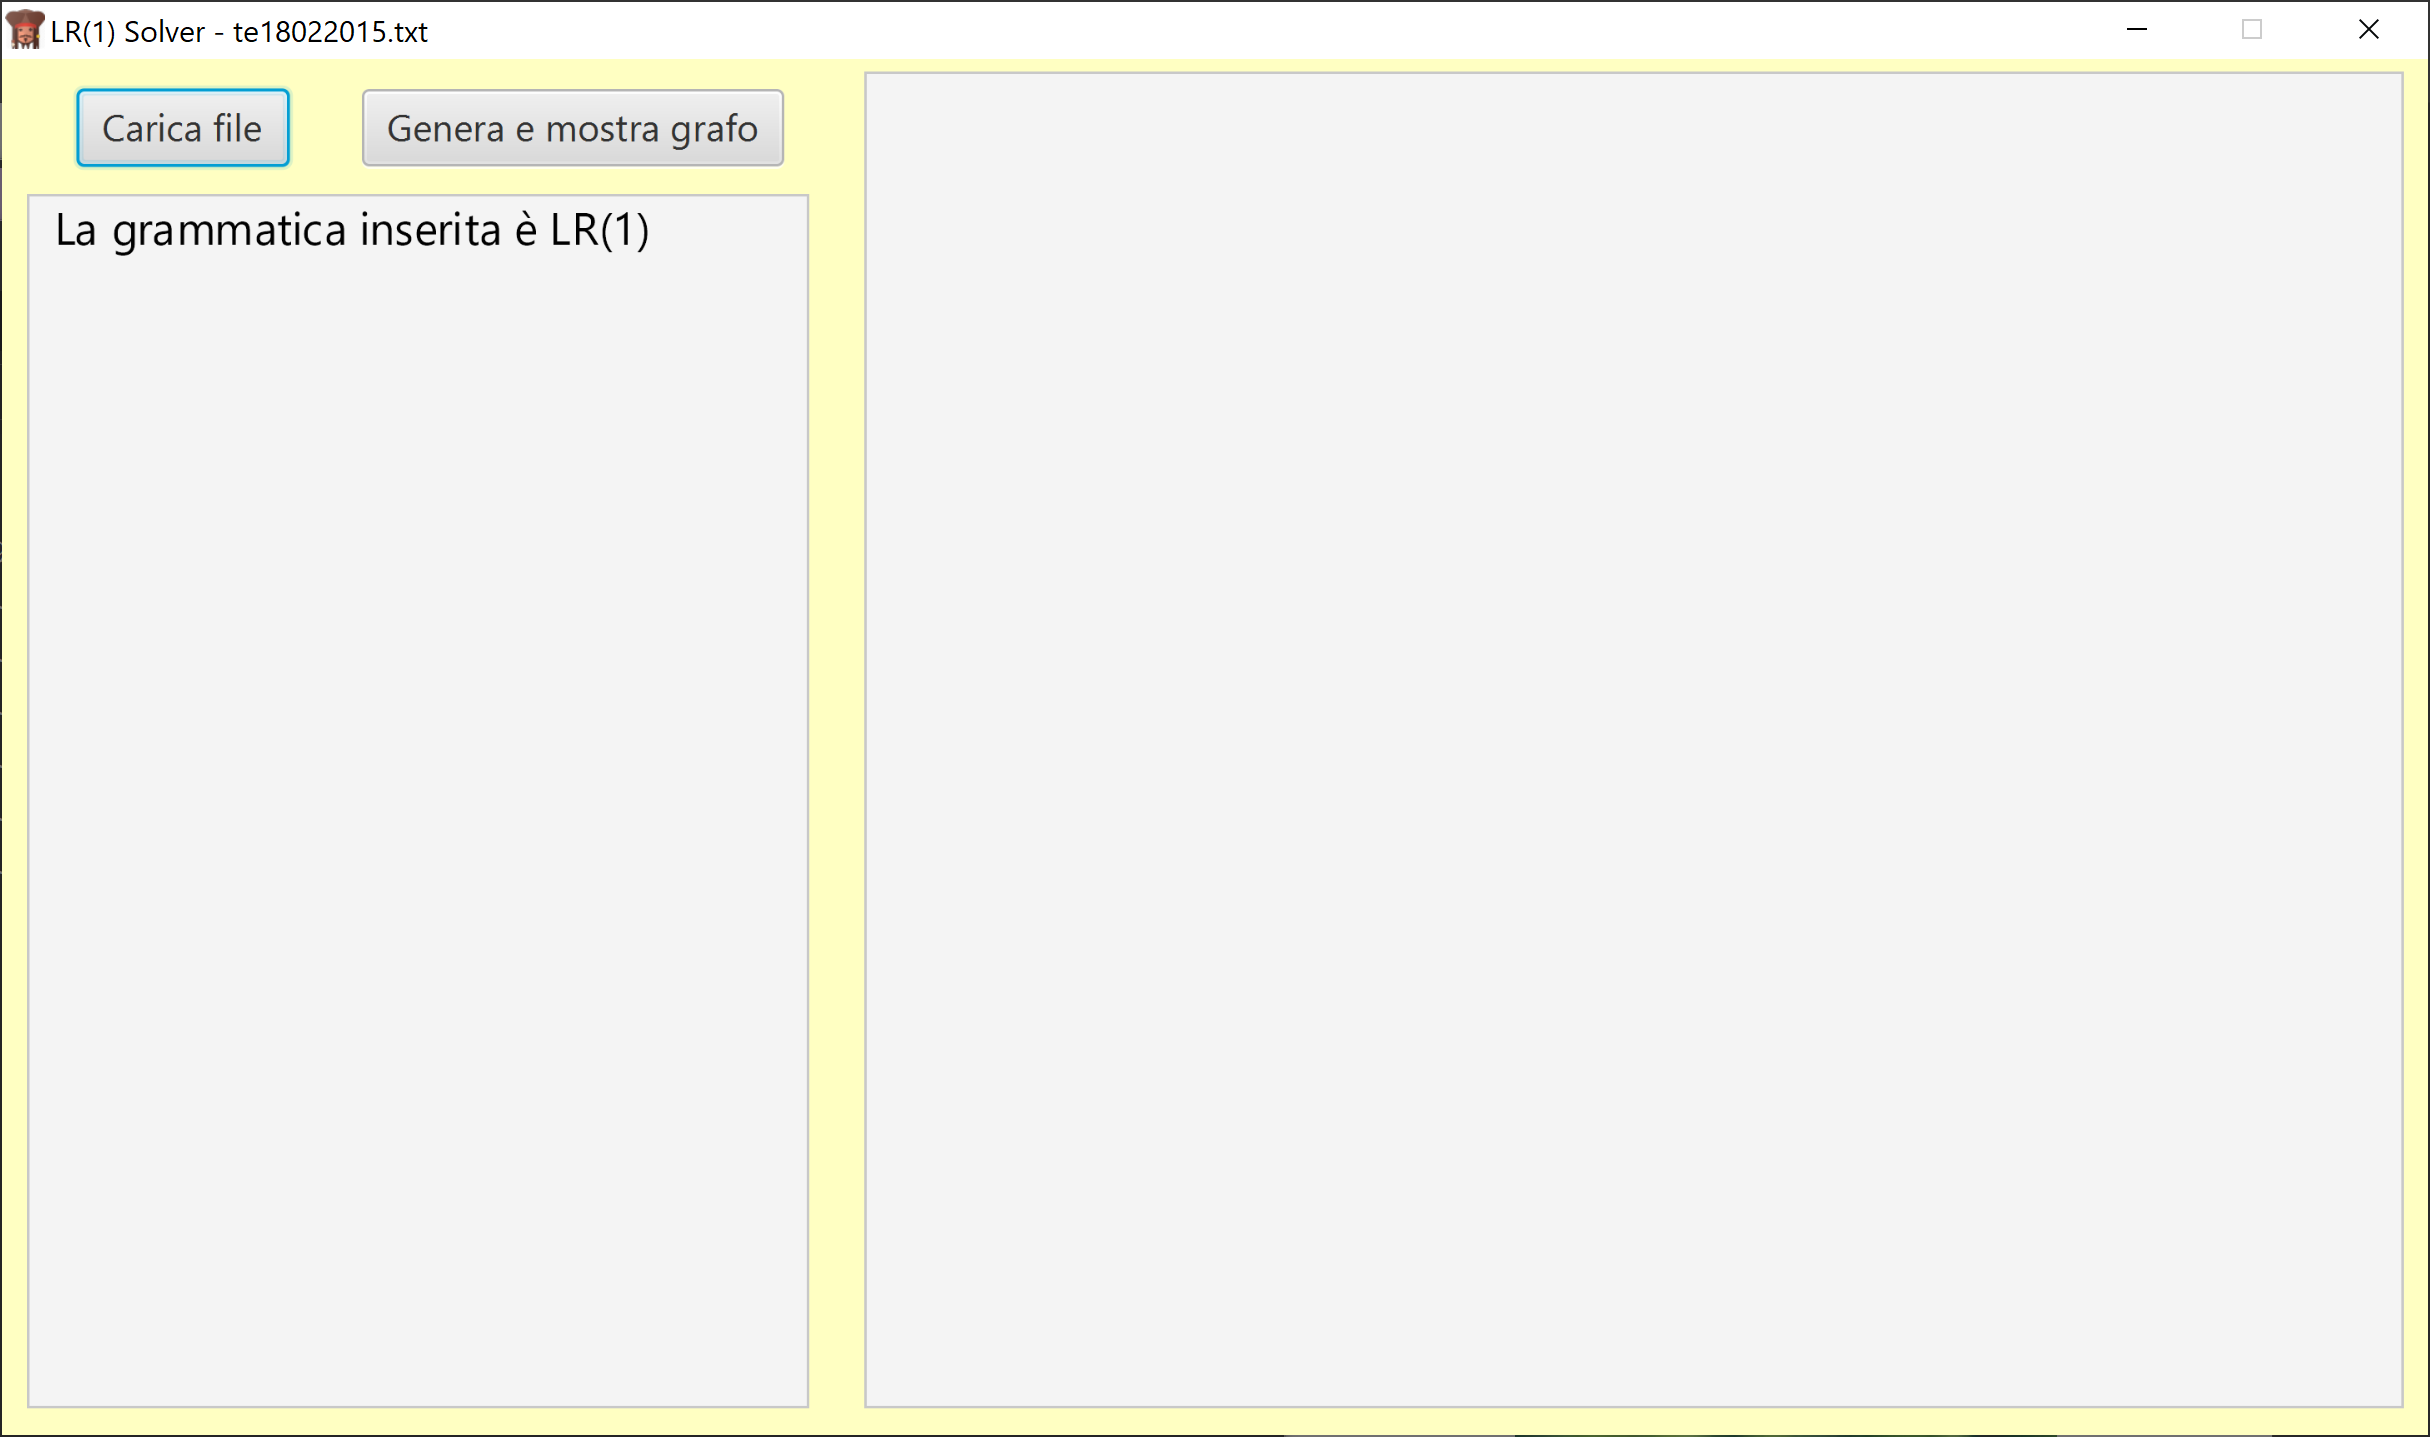
\includegraphics[scale=0.5]{immagini/GrammaticaLR1.png}
\caption{Finestra con messaggio grammatica LR(1)}
\end{figure}

\subsection{Esempio grammatica non LR(1)}
Se la grammatica inserita non è di tipo LR(1) verrà visualizzato un messaggio come il seguente, dove verranno inoltre riportati i nomi degli stati in errore:
\begin{figure}[h!]
\centering
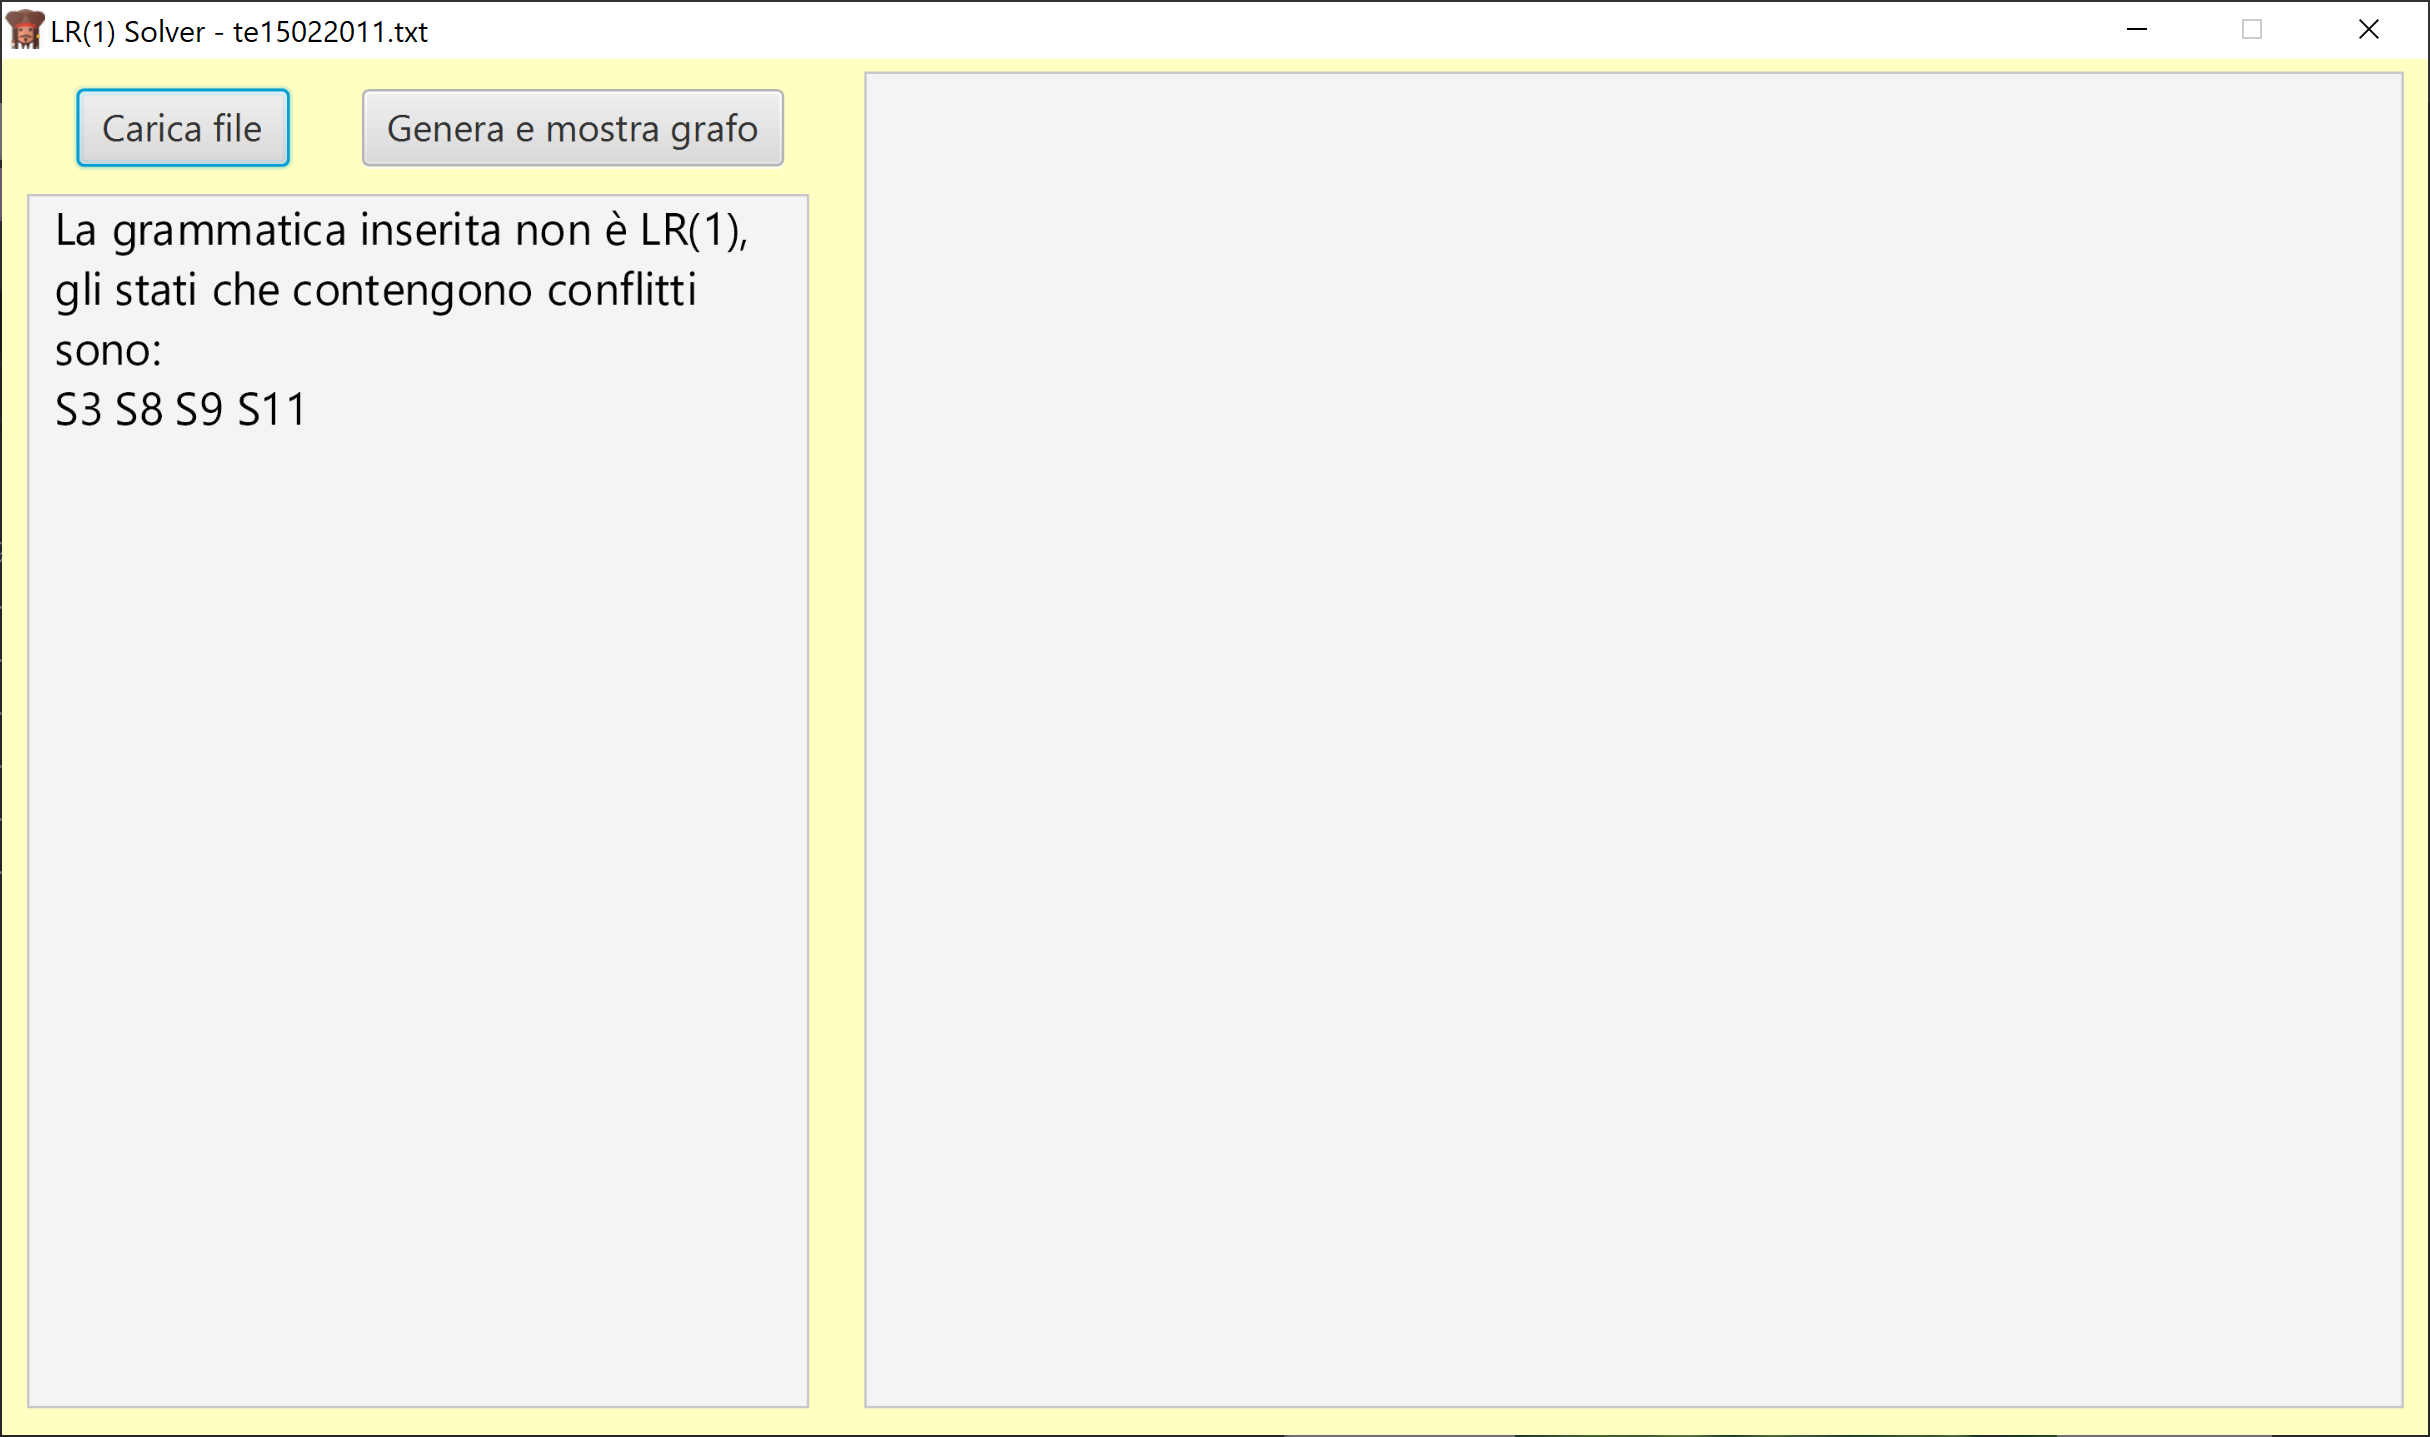
\includegraphics[scale=0.5]{immagini/GrammaticaNoLR1.png}
\caption{Finestra con messaggio grammatica non LR(1)}
\end{figure}
\pagebreak

\subsection{Esempio grammatica con errori}
Se la grammatica inserita contiene errori verrà visualizzato un messaggio con il tipo di errore presente:
\begin{figure}[h!]
\centering
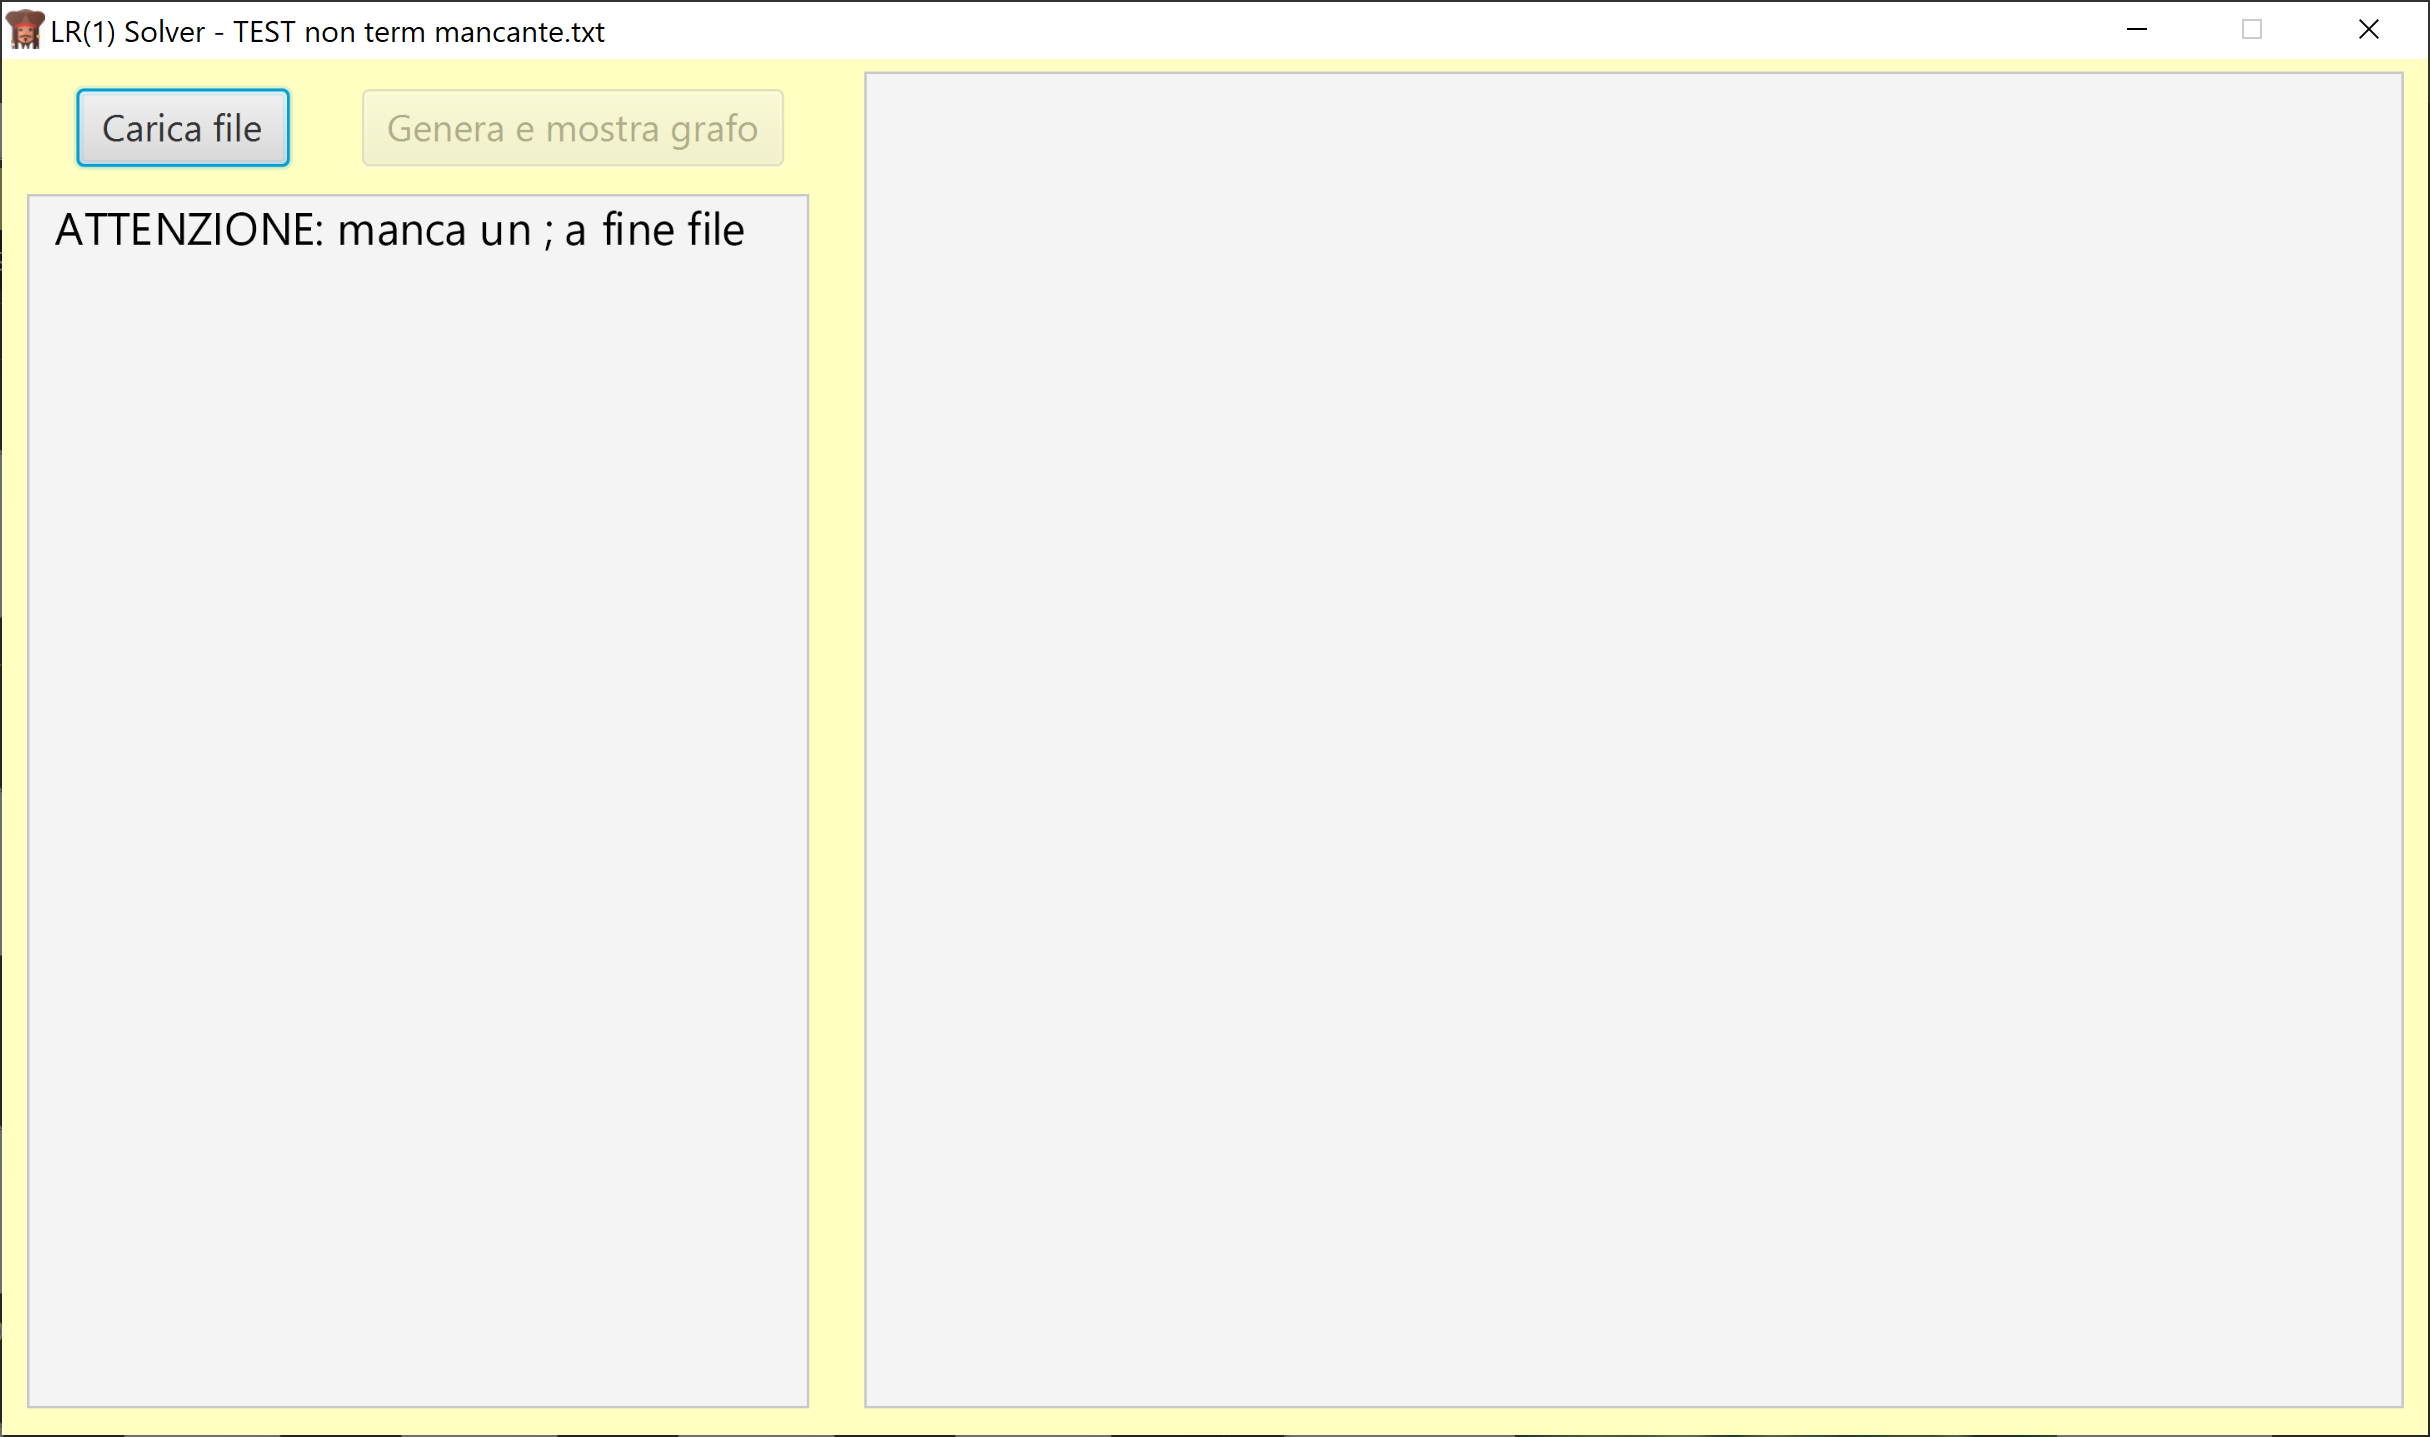
\includegraphics[scale=0.5]{immagini/GrammaticaErrata.png}
\caption{Finestra con messaggio grammatica errata}
\end{figure}

Se il tipo di errore è risolvibile automaticamente dal programma, verrà mostrato se la grammatica è o non è di tipo LR(1) oltre al tipo di errore presente.
\begin{figure}[h!]
\centering
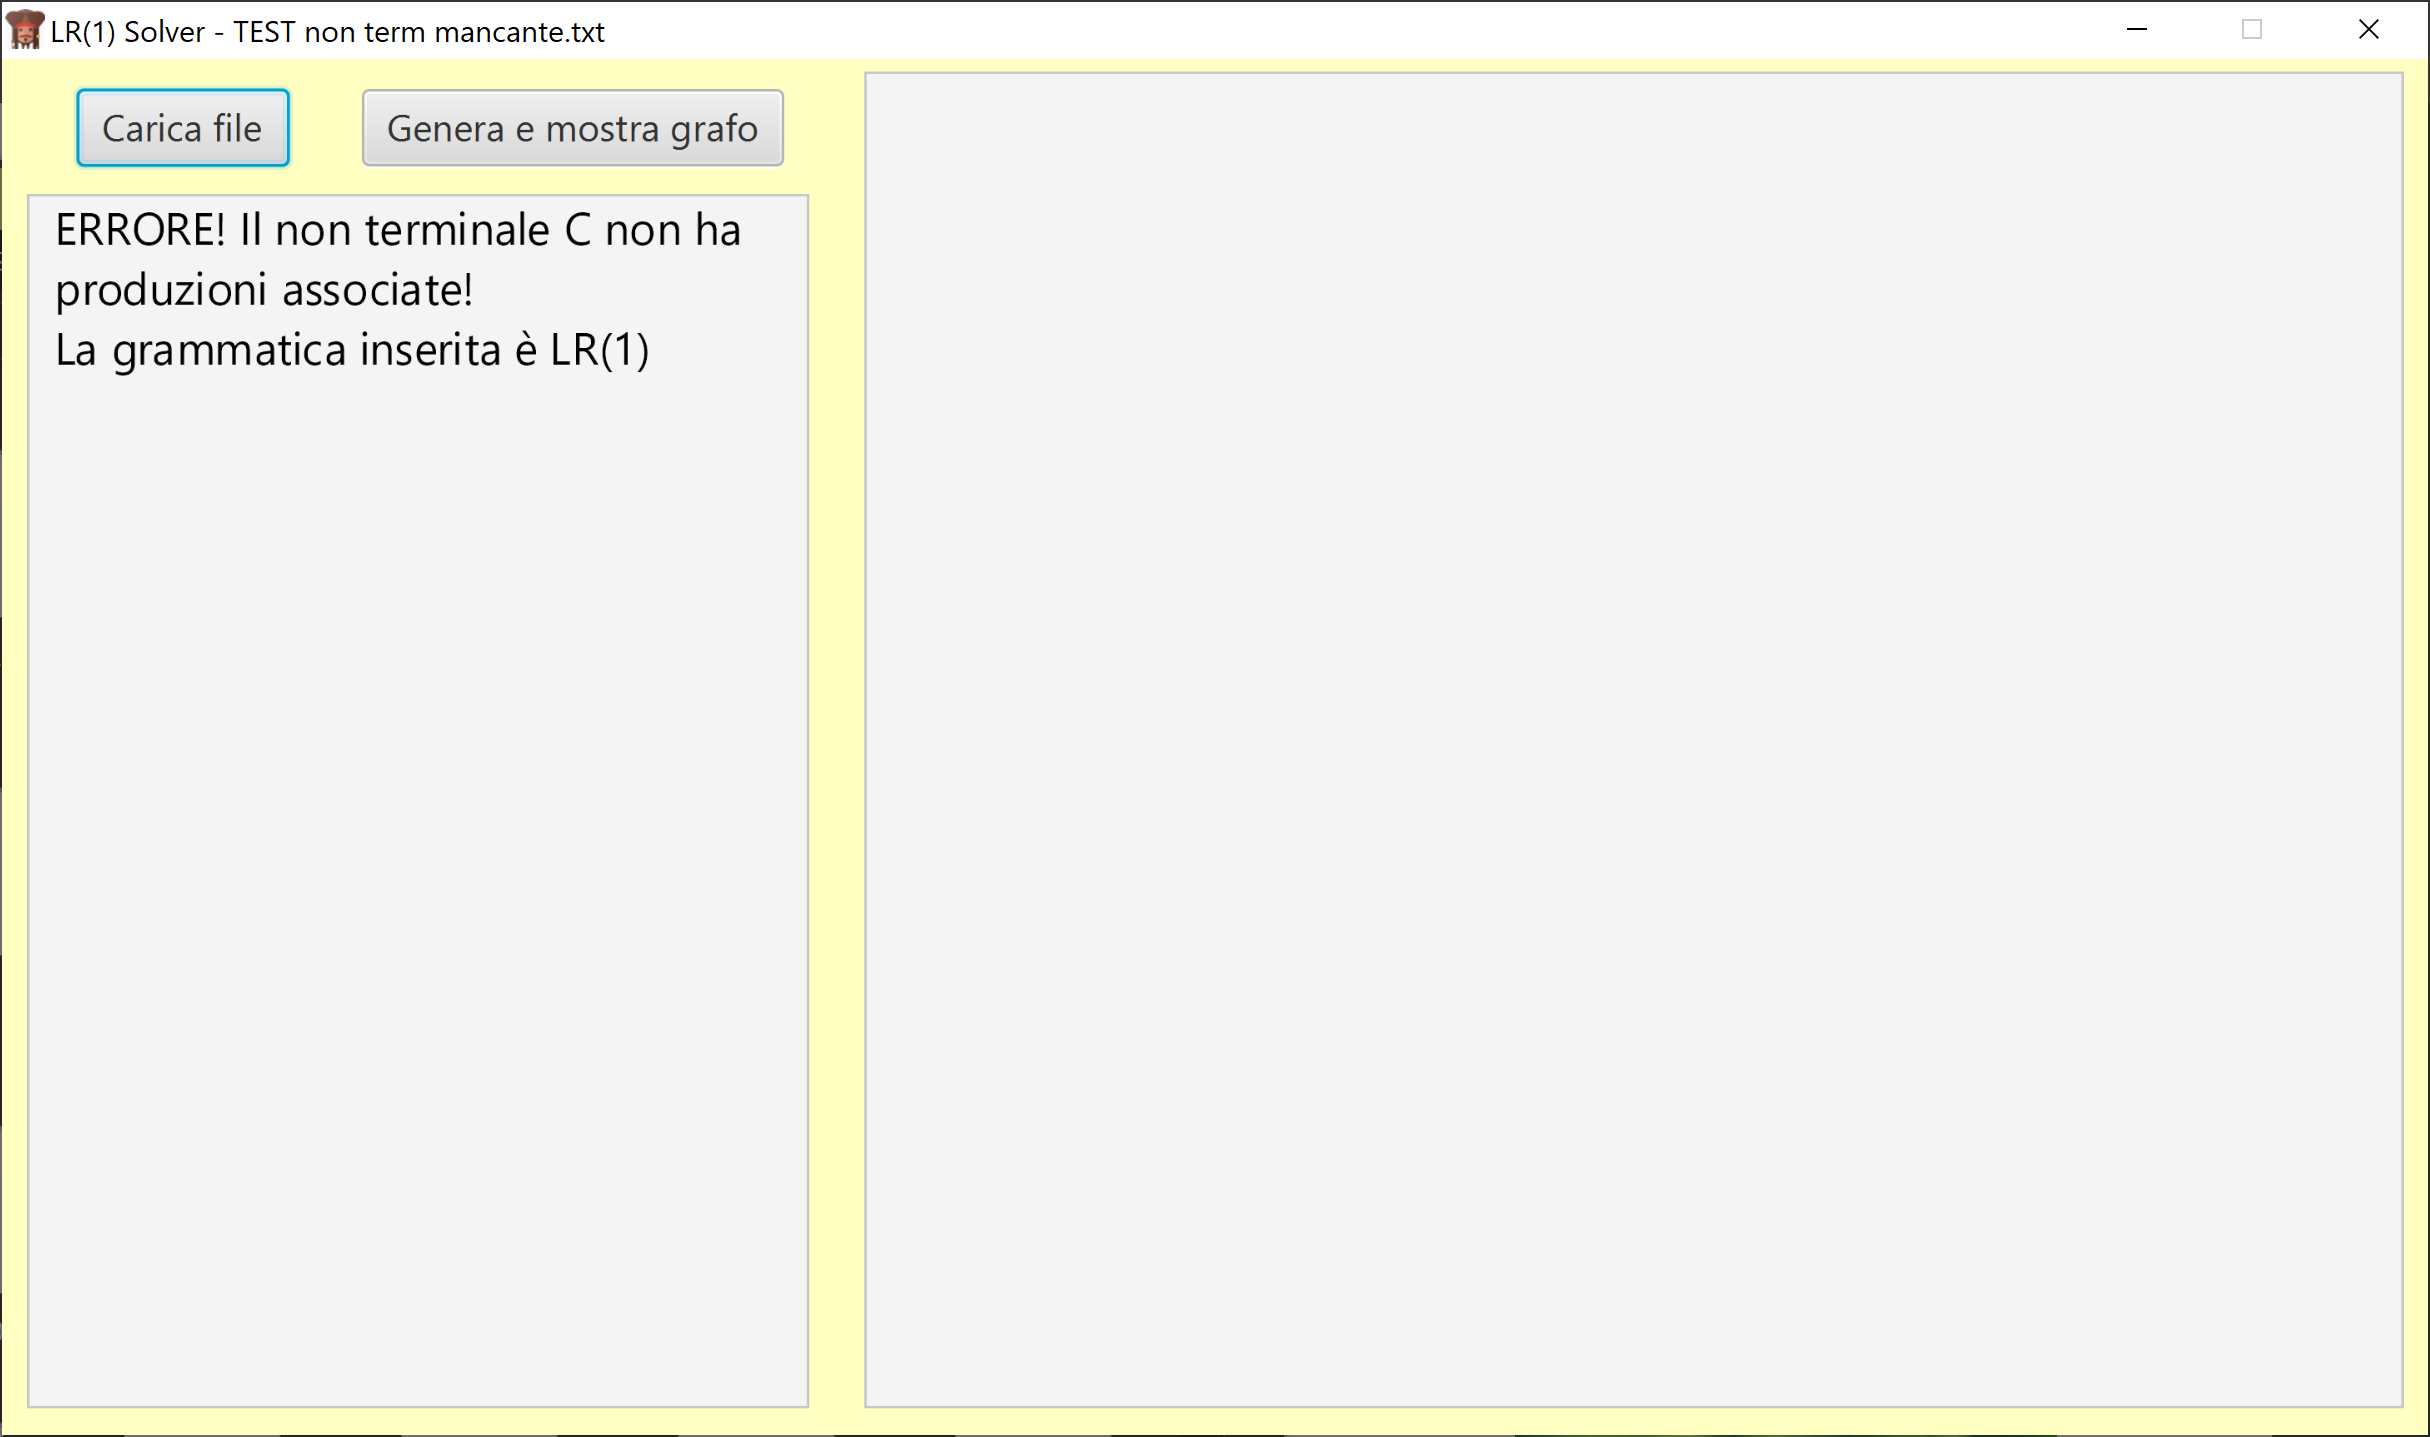
\includegraphics[scale=0.5]{immagini/GrammaticaErrataRis.png}
\caption{Finestra con messaggio grammatica LR(1), ma errata}
\end{figure}
\pagebreak

\subsection{Generazione e salvataggio del grafo}
Una volta analizzata la grammatica, se essa non presenta errori bloccanti, sarà possibile, premendo l'apposito tasto in alto, generare e mostrare il grafo.
Una volta premuto il tasto si aprirà una finestra, come la seguente, per scegliere dove salvare l'immagine generata (può essere salvata sia in .jpg che .png):
\begin{figure}[h!]
\centering
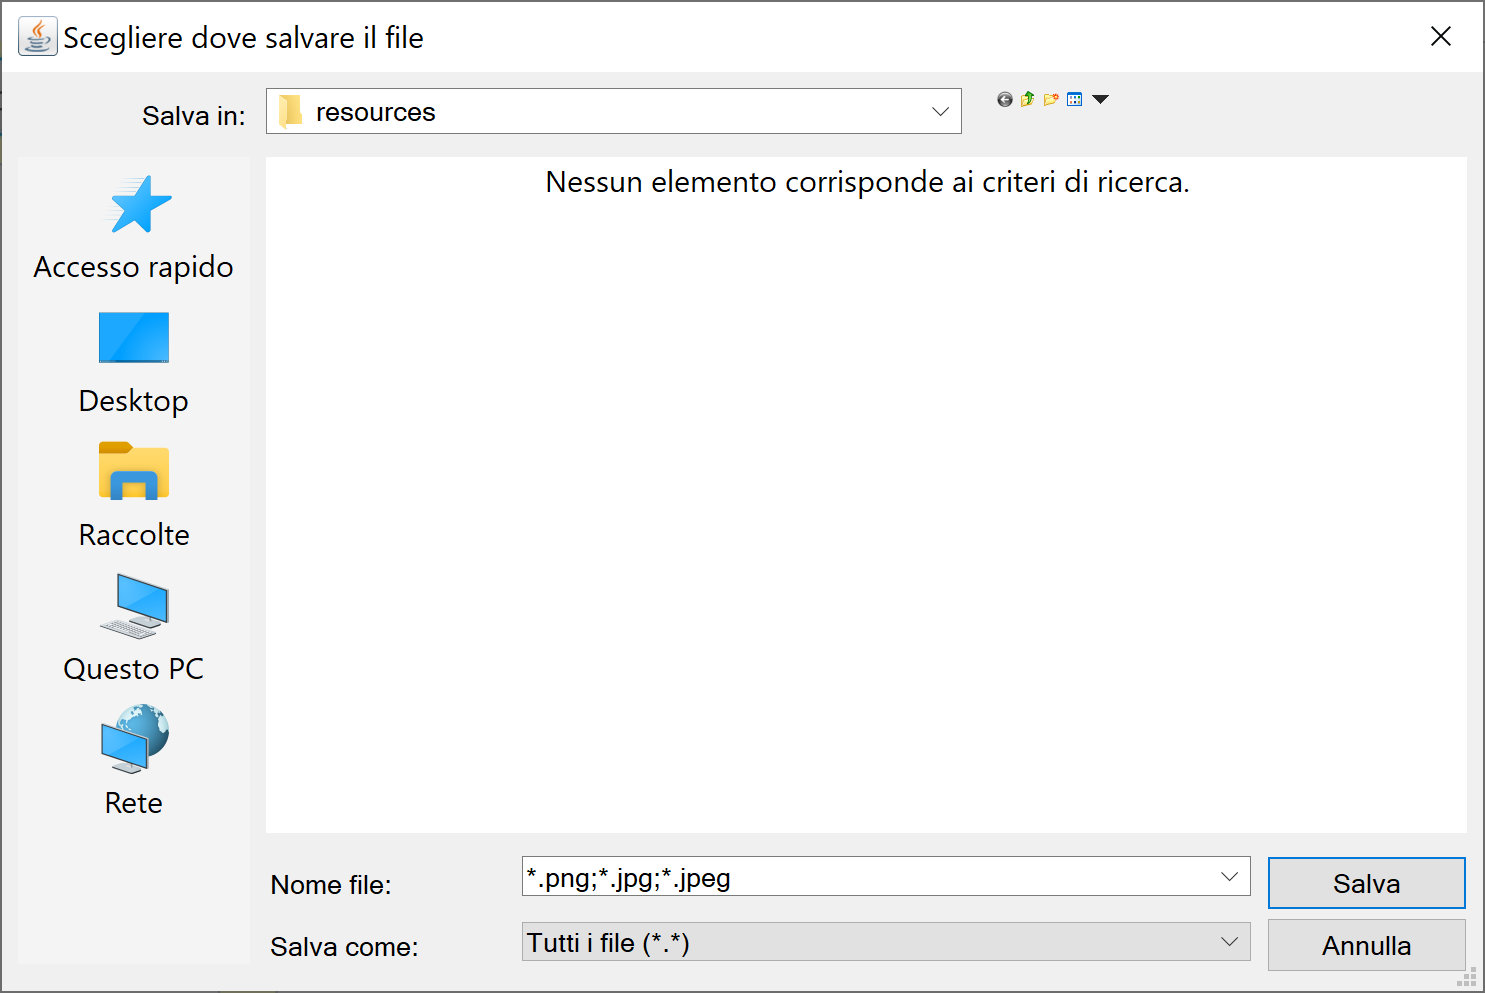
\includegraphics[scale=0.6]{immagini/SalvaImmagine.png}
\caption{Finestra di salvataggio immagine grafo}
\end{figure}

A questo punto nella parte destra del programma verrà visualizzata l'immagine del grafo:
\begin{figure}[h!]
\centering
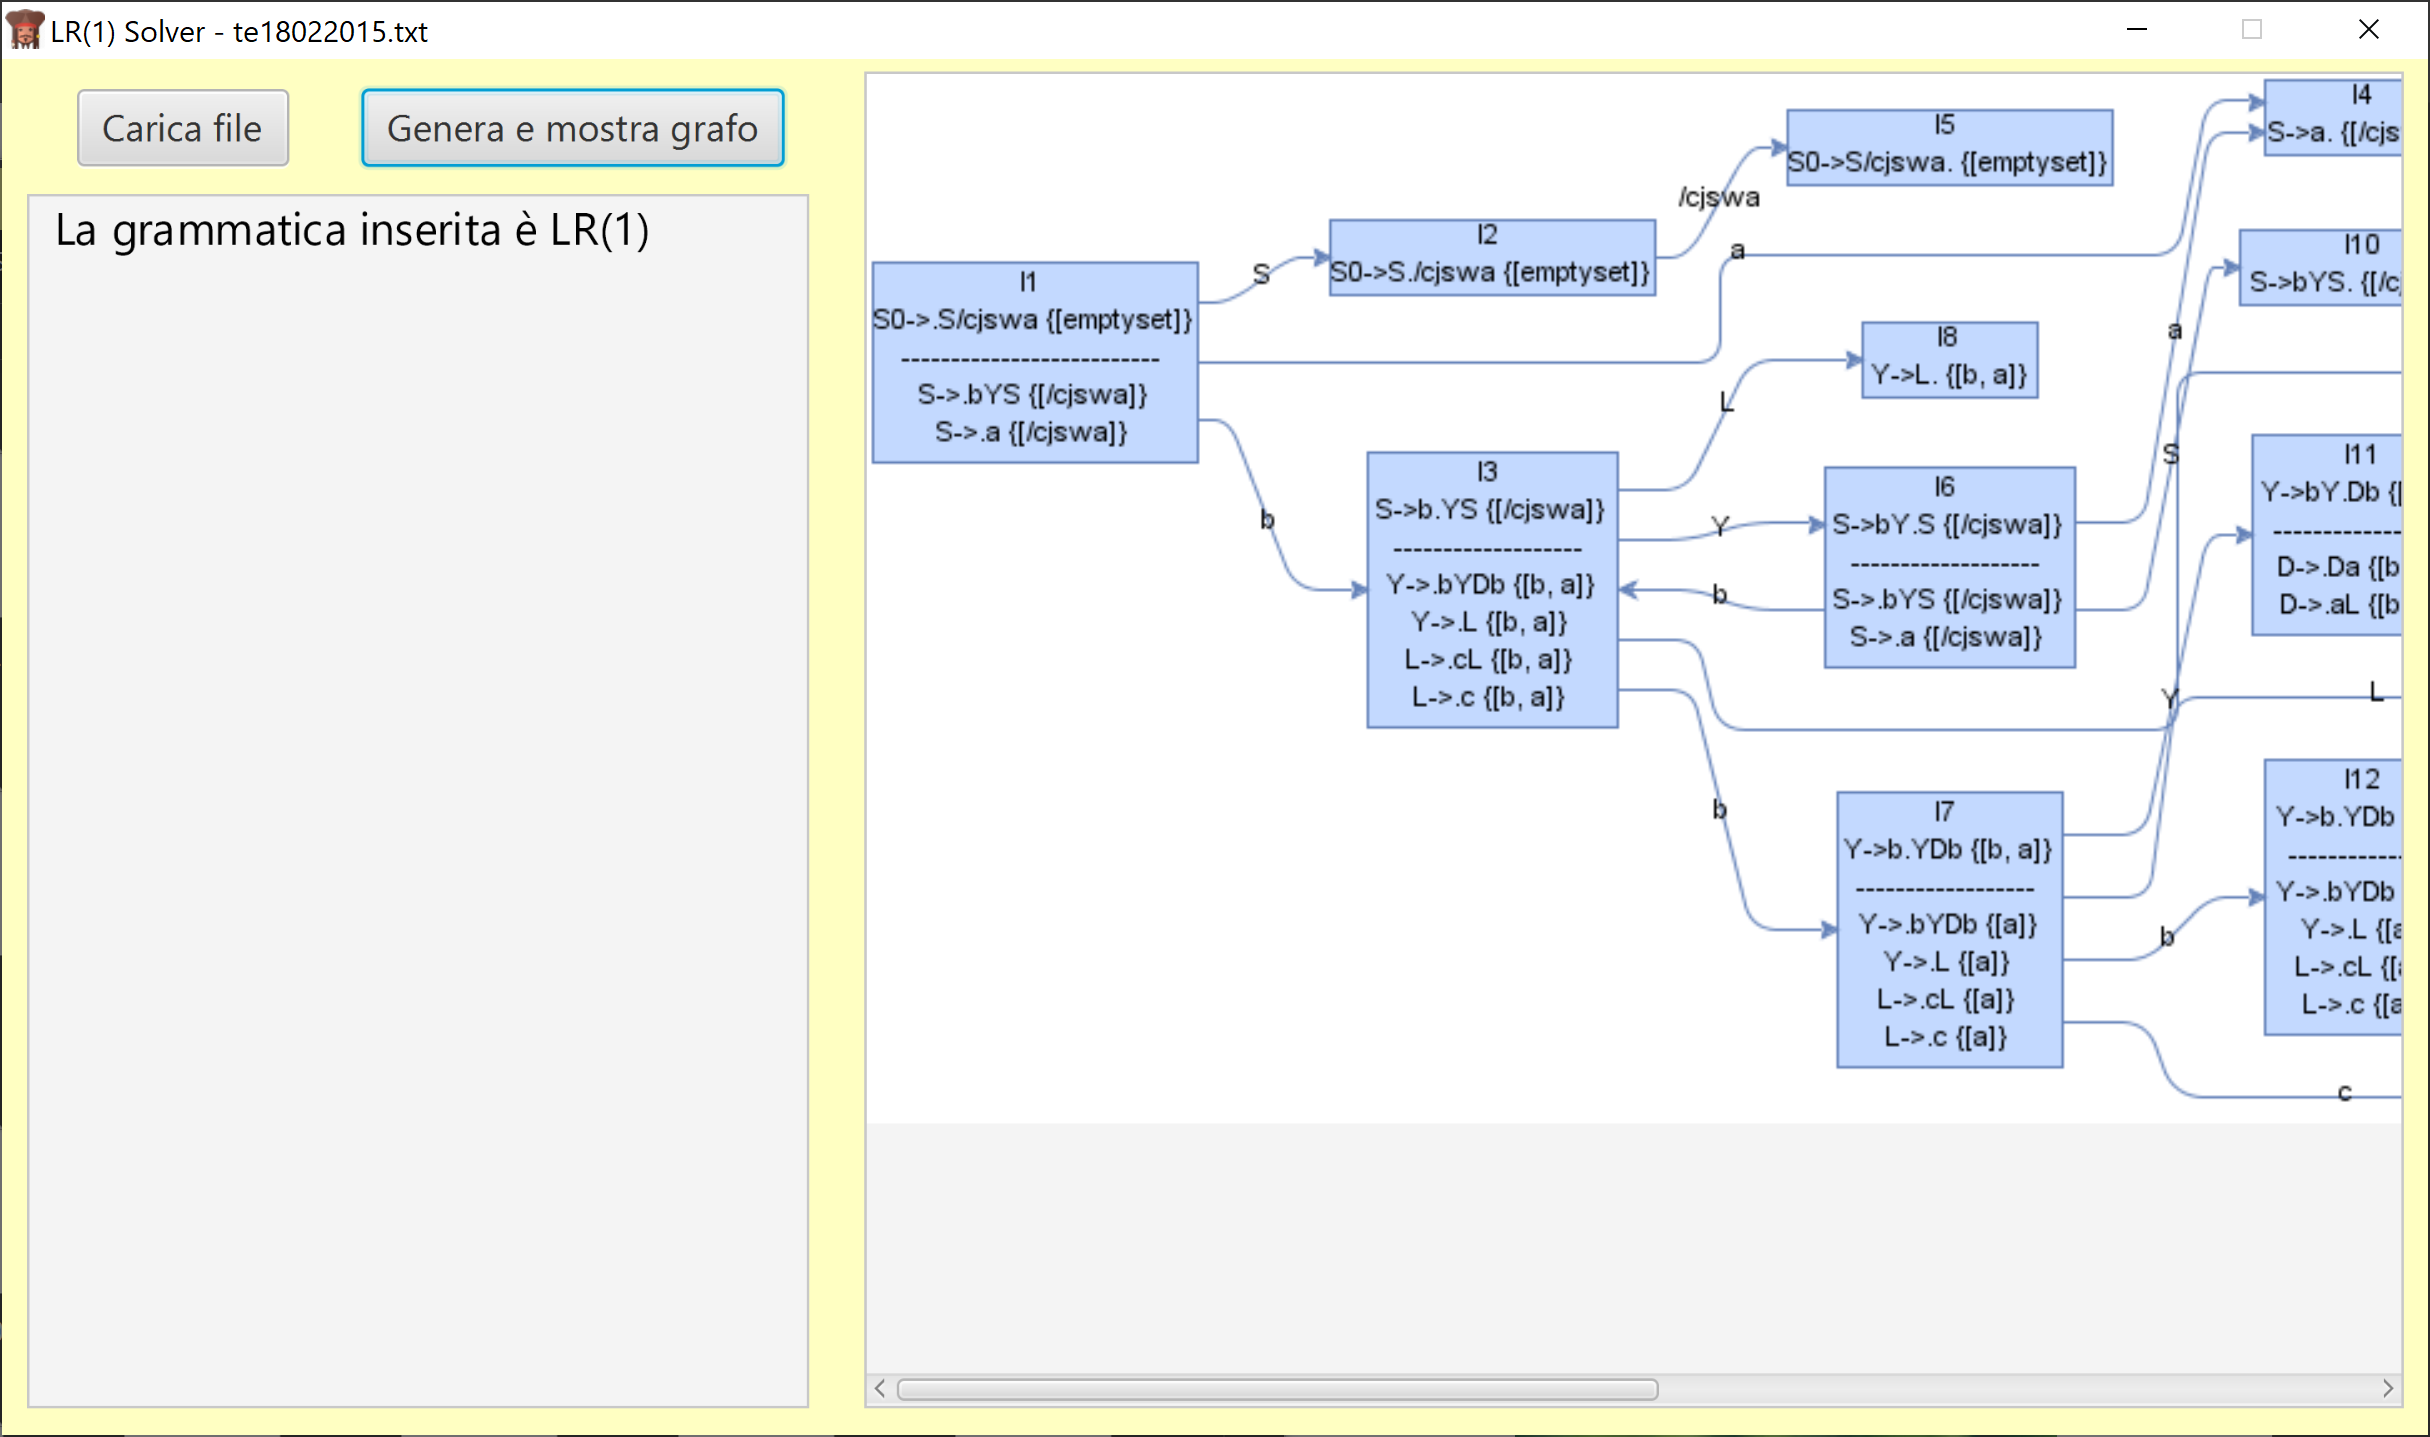
\includegraphics[scale=0.5]{immagini/GrammaticaLR1Immagine.png}
\caption{Grafo di una grammatica LR(1)}
\end{figure}
\pagebreak

Se qualche stato dovesse invece presentare errori, essi sarebbero colorati di rosso:
\begin{figure}[h!]
\centering
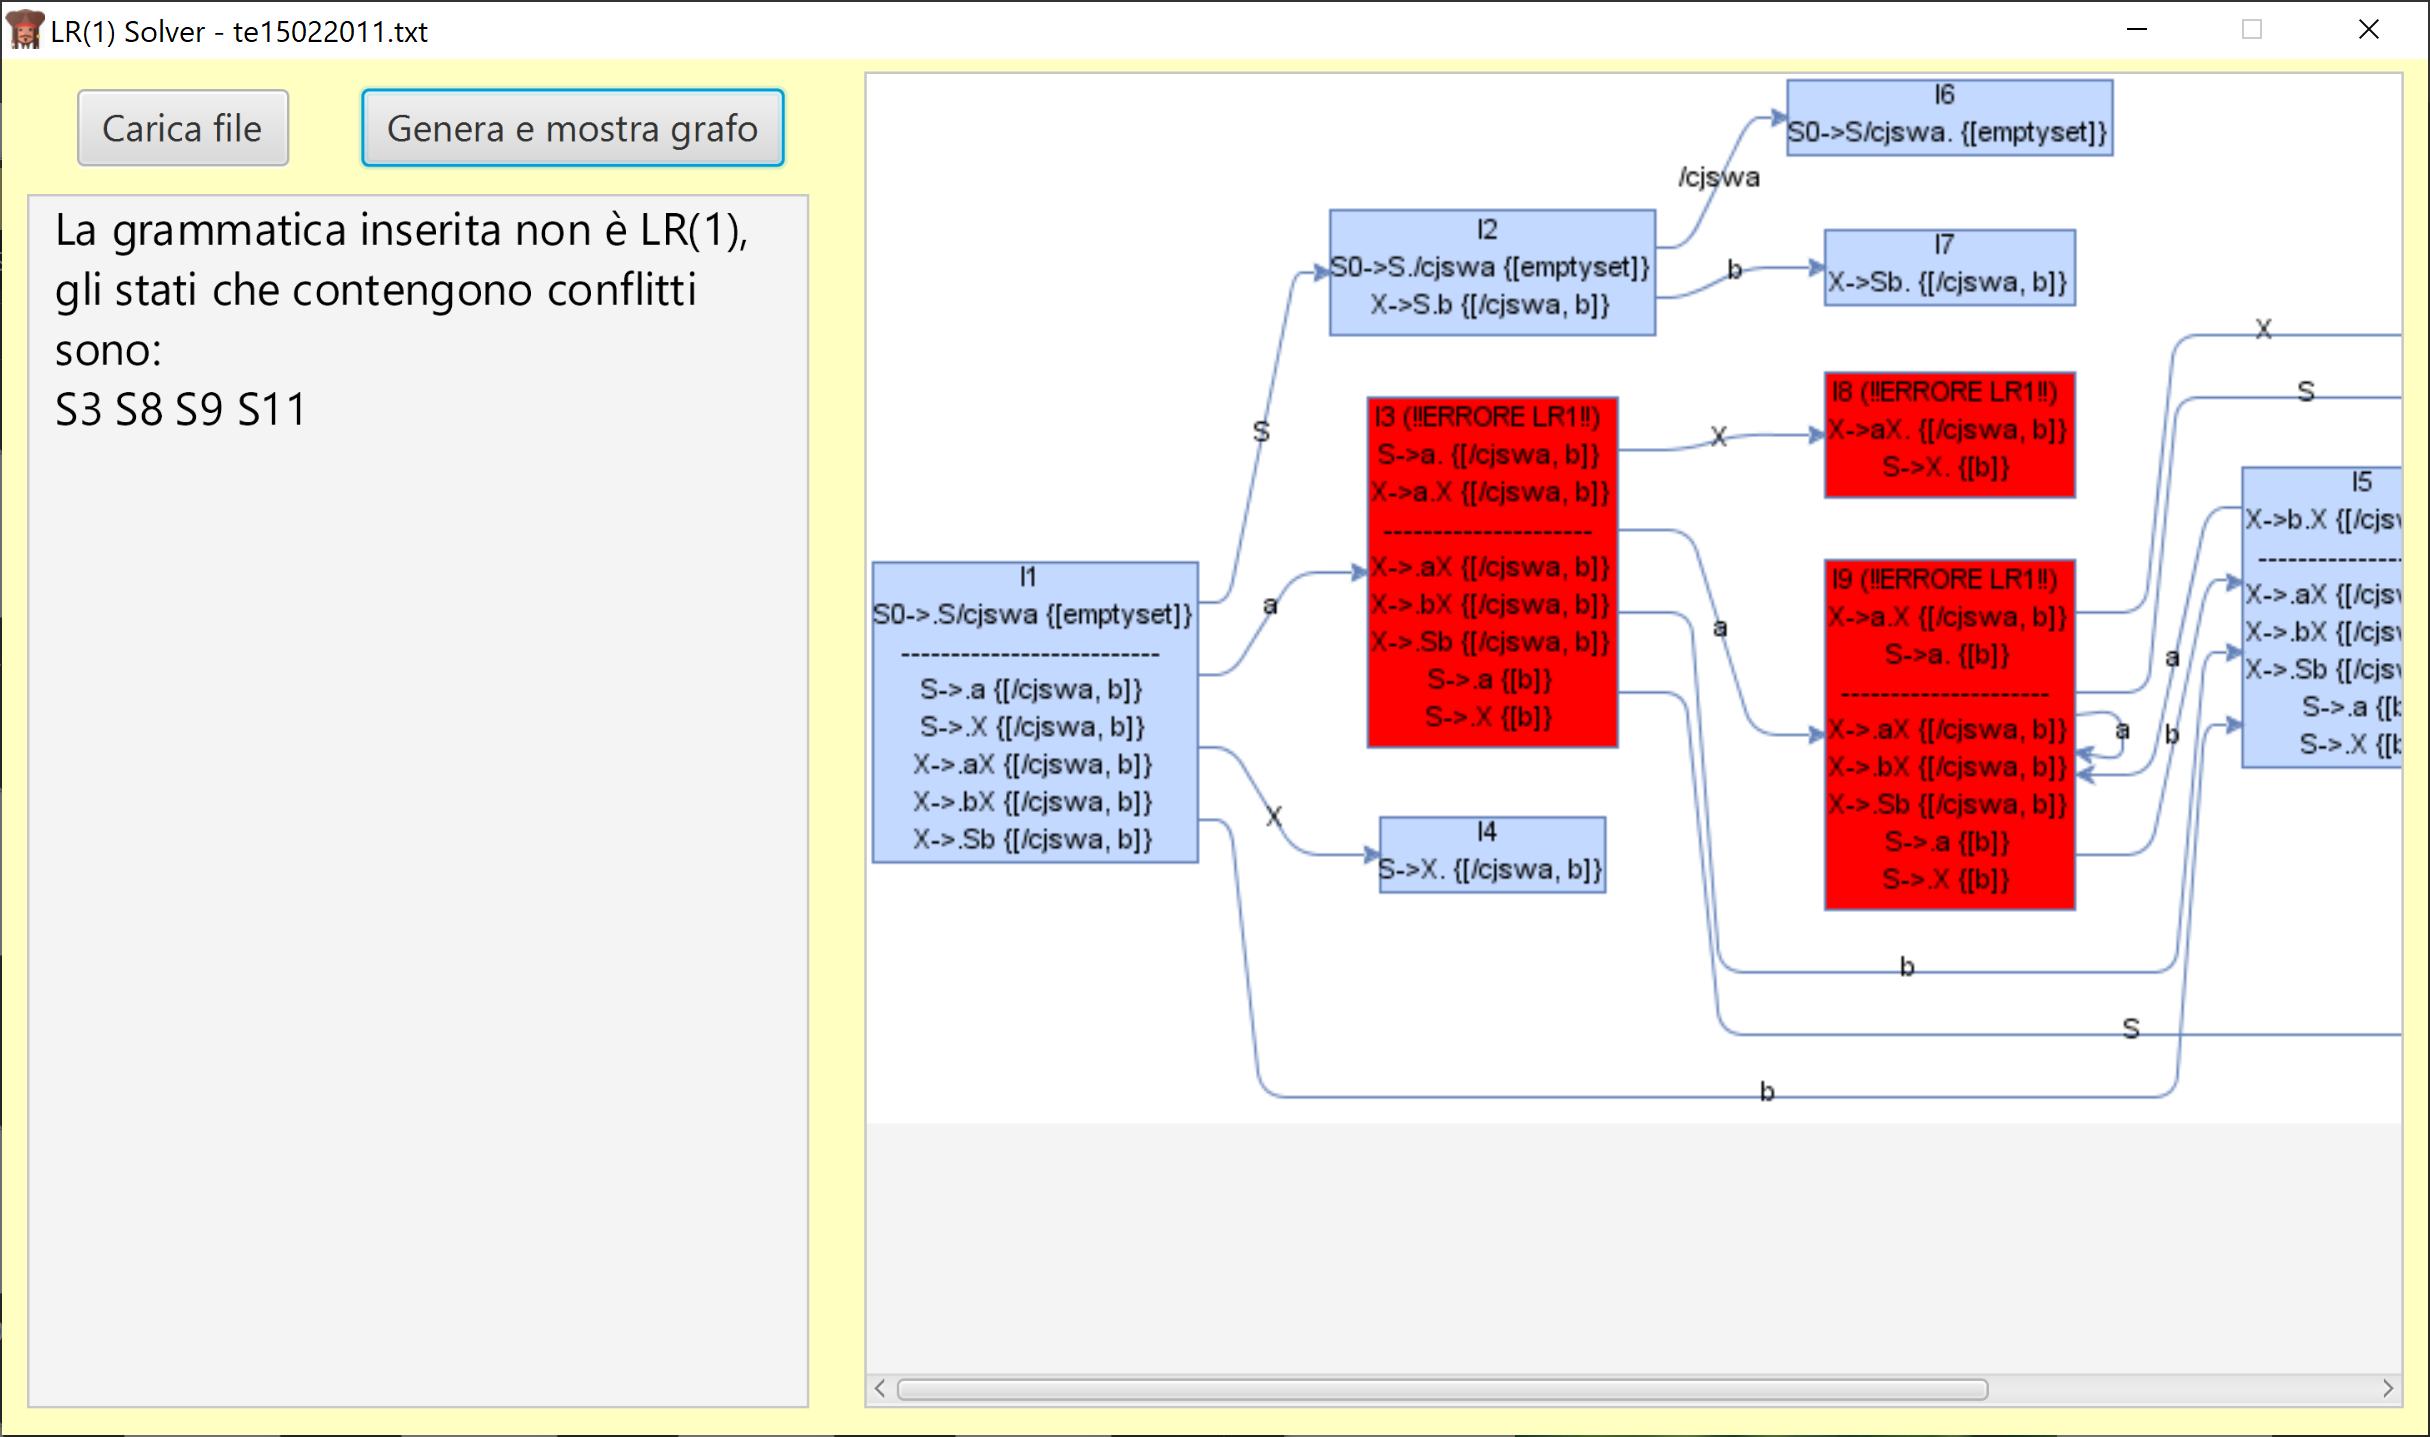
\includegraphics[scale=0.5]{immagini/GrammaticaNoLR1Immagine.png}
\caption{Grafo di una grammatica non LR(1)}
\end{figure}

\end{document}